% 1977 年吉林卷第 5 题：测距示意——四边形 ABCD，
% 基线 CD=200，C 处标 105°、15°，D 处标 30°、120°（按源卷第 3 页布局：A、B 在上）
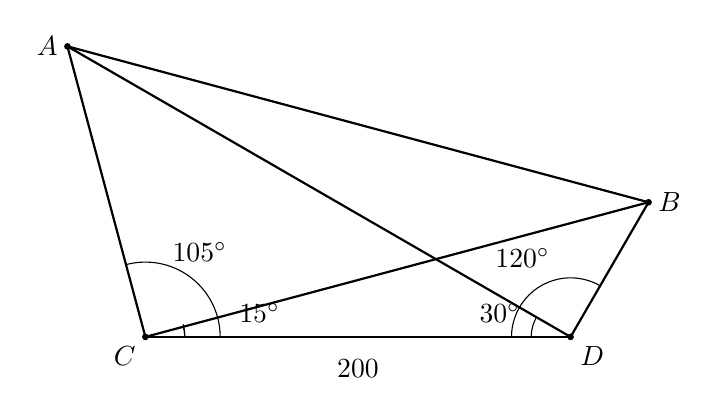
\begin{tikzpicture}[scale=1.0]
  \coordinate (C) at (0,0);
  \coordinate (D) at (5.4,0);
  \coordinate (A) at (-0.99,3.69);
  \coordinate (B) at (6.39,1.71);
  \draw[thick] (A)--(B);
  \draw[thick] (A)--(C);
  \draw[thick] (A)--(D);
  \draw[thick] (B)--(C);
  \draw[thick] (B)--(D);
  \draw[thick] (C)--(D);
  \draw (0.95,0) arc[start angle=0,end angle=105,radius=0.95];
  \draw (0.5,0) arc[start angle=0,end angle=15,radius=0.5];
  \draw (0.5,0) arc[start angle=0,end angle=15,radius=0.62];
  \draw ([shift=(180:0.5)]D) arc[start angle=180,end angle=150,radius=0.5];
  \draw ([shift=(180:0.75)]D) arc[start angle=180,end angle=60,radius=0.75];
  \fill (A) circle (1.2pt) node[left] {$A$};
  \fill (B) circle (1.2pt) node[right] {$B$};
  \fill (C) circle (1.2pt) node[below left] {$C$};
  \fill (D) circle (1.2pt) node[below right] {$D$};
  \node at (0.69,1.08) {$105^\circ$};
  \node at (1.45,0.30) {$15^\circ$};
  \node at (4.5,0.30) {$30^\circ$};
  \node at (4.79,1.00) {$120^\circ$};
  \node at (2.7,-0.4) {$200$};
\end{tikzpicture}
